\hypertarget{group__Reporter}{\section{Reporter}
\label{group__Reporter}\index{Reporter@{Reporter}}
}


\mbox{[}Ordering 600\mbox{]} Report tests results stage  


Collaboration diagram for Reporter\-:
\nopagebreak
\begin{figure}[H]
\begin{center}
\leavevmode
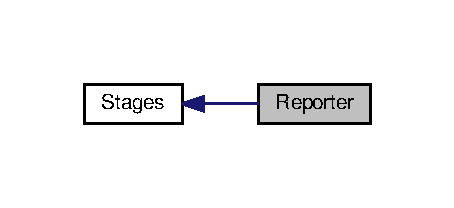
\includegraphics[width=218pt]{group__Reporter}
\end{center}
\end{figure}
\mbox{[}Ordering 600\mbox{]} Report tests results stage \hypertarget{group__Reporter_IUDatabase}{}\subsection{I\-U\-Database}\label{group__Reporter_IUDatabase}
M\-T\-T Database reporter plugin for the legacy I\-U submission server 
\begin{DoxyParams}{Parameters}
{\em realm} & Database name \\
\hline
{\em username} & Username to be used for submitting data \\
\hline
{\em password} & Password for that username \\
\hline
{\em pwfile} & File where password can be found \\
\hline
{\em platform} & Name of the platform (cluster) upon which the tests were run \\
\hline
{\em hostname} & Name of the hosts involved in the tests (may be regular expression) \\
\hline
{\em url} & U\-R\-L of the database server \\
\hline
{\em debug\-\_\-filename} & Debug output file for server interaction information \\
\hline
{\em keep\-\_\-debug\-\_\-files} & Retain reporter debug output after execution \\
\hline
{\em debug\-\_\-server} & Ask the server to return its debug output as well \\
\hline
{\em email} & Email to which errors are to be sent\\
\hline
\end{DoxyParams}
\hypertarget{group__Reporter_JunitXML}{}\subsection{Junit\-X\-M\-L}\label{group__Reporter_JunitXML}
Junit X\-M\-L plugin 
\begin{DoxyParams}{Parameters}
{\em filename} & Name of the file into which the report is to be written \\
\hline
{\em textwrap} & Max line length before wrapping\\
\hline
\end{DoxyParams}
\hypertarget{group__Reporter_TextFile}{}\subsection{Text\-File}\label{group__Reporter_TextFile}
File reporter plugin 
\begin{DoxyParams}{Parameters}
{\em filename} & Name of the file into which the report is to be written \\
\hline
{\em summary\-\_\-footer} & Footer to be placed at bottom of summary \\
\hline
{\em detail\-\_\-header} & Header to be put at top of detail report \\
\hline
{\em detail\-\_\-footer} & Footer to be placed at bottome of detail report \\
\hline
{\em textwrap} & Max line length before wrapping \\
\hline
\end{DoxyParams}
